\question This problem is for extra credit and is worth 1/2 of a regular problem.

A loop of wire with dimensions $h\times w$ rotates about its central axis with an angular frequency $\omega$. The wire is in the presence of a uniform magnetic field which points in the upward direction at all times. If $w=10$ cm, $h=15$ cm, $|\vec{B}|=0.2$ T, and $\omega=400$ s$^{-1}$, what is the maximum emf generated around the loop?

\begin{figure}[ht!]
	\centering
	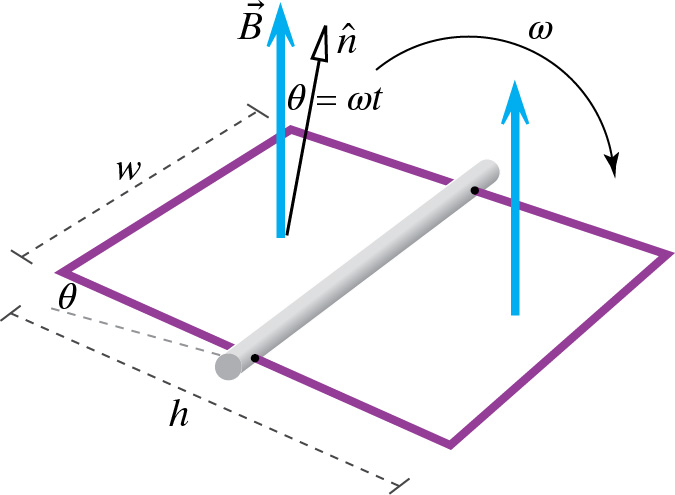
\includegraphics[width=8cm]{examfig.jpg}
\end{figure}